\documentclass[10pt,letterpaper,twocolumn]{article}
%\documentclass[10pt,letterpaper]{article}
% ---------------------------------------------------------------
\usepackage[utf8]{inputenc}
\usepackage[spanish]{babel}
\usepackage{listings}
\usepackage[usenames,dvipsnames]{color}
\usepackage{amsmath}
\usepackage{calc}
\usepackage{verbatim}
\usepackage{hyperref}
\usepackage{color}
\usepackage{geometry}
\usepackage[pdftex]{graphicx}
\usepackage{pgfplots}
\usepackage{array}

\usetikzlibrary{external}
\tikzexternalize[prefix=pics/]

% Para incluir gráficas en MetaPost: http://tex.stackexchange.com/questions/1565/metapost-pictures-in-pdflatex
\DeclareGraphicsRule{.1}{mps}{*}{} 
\DeclareGraphicsRule{.2}{mps}{*}{}
\DeclareGraphicsRule{.3}{mps}{*}{}
\DeclareGraphicsRule{.4}{mps}{*}{}

%Poner la página en landscape
\geometry{verbose,landscape,letterpaper,tmargin=1.5cm,bmargin=2cm,lmargin=1.6cm,rmargin=1.6cm}

\newcommand{\codigofuente}[1]{
\verbatiminput{#1}
\dotfill
}
\setlength{\columnsep}{0.25in}
\setlength{\columnseprule}{1px}

% ---------------------------------------------------------------
\begin{document}
% ---------------------------------------------------------------
\title{Resumen de algoritmos para torneos de programación}
\author{Andrés Mejía}
\date{\today}
\maketitle
% ---------------------------------------------------------------

% ---------------------------------------------------------------
\tableofcontents
% ---------------------------------------------------------------
\section{Plantilla}
\codigofuente{./src/template.cpp}
% ---------------------------------------------------------------
\section{Teoría de números}
% ---------------------------------------------------------------
\subsection{Big mod}
\codigofuente{./src/teoria_de_numeros/bigmod.cpp}

\subsection{Criba de Eratóstenes}
\small
\textbf{Field-testing:}
\begin{itemize}
\item \emph{SPOJ} -  2912 - Super Primes
\item \emph{Live Archive} - 3639 - Prime Path
\end{itemize}

\normalsize
Marca los números primos en un arreglo. Algunos tiempos de ejecución:
\begin{center}
  \begin{tabular}{c c}
    \hline\hline
    SIZE & Tiempo (s) \\ [0.5ex]
    \hline
    100000 & 0.007 \\
    1000000 & 0.032 \\
    10000000 & 0.253 \\
    100000000 & 2.749 \\ [1ex]
    \hline
  \end{tabular}
\end{center}
\codigofuente{./src/teoria_de_numeros/criba.cpp}

\subsection{Divisores de un número}
Imprime todos los divisores de un número (en desorden) en O($\sqrt{n}$).
Hasta 4294967295 (máximo \textit{unsigned int}) responde instantáneamente. Se puede
forzar un poco más usando \textit{unsigned long long} pero más allá de $10^{12}$ empieza a
responder muy lento.
\codigofuente{./src/teoria_de_numeros/divisores.cpp}

Si sólo se requiere contar los divisores, usando la criba de Eratóstenes se puede usar esta propiedad:
\begin{quote}
Si la descomposición prima de $n > 1$ es $$n = p_0^{e_0} \times p_1^{e_1} \times \cdots \times p_{n}^{e_n}$$ entonces el número de divisores (positivos) de $n$ es $$(e_0 + 1) \times (e_1 + 1) \times \cdots \times (e_n + 1).$$
\end{quote}


\subsection{Propiedades modulares y algunas identidades}

\begin{itemize}
  \item $ a \mid c \land b \mid c \land gcd(a, b) = 1 \rightarrow ab \mid c $
  \item \textbf{Euclid's Lemma:}  $ a \mid bc \land gcd(a, b) = 1 \rightarrow a \mid c $
  \item $ x^n - 1 = (x - 1)(x^{n - 1} + x^{n - 2} + \cdots + x + 1) $
\end{itemize}

\subsection{Inverso modular}

El inverso modular de $a \bmod{n}$ es un entero denotado por $a^{-1}$ tal que $a (a^{-1}) \equiv 1 \pmod{n}$. Existe si y sólo si $gcd(a, n) == 1$.

Si el inverso módulo $n$ existe, la operación de dividir por $a \bmod{n}$ se puede definir como multiplicar por el inverso.

\codigofuente{./src/teoria_de_numeros/inverso_modular.cpp}

\subsection{Teorema chino del residuo}

Sean $b_1, b_2, \cdots, b_{r}$ enteros positivos primos relativos dos a dos. Llamemos $B = b_1 b_2 \cdots b_r$. El sistema de congruencias lineales
\begin{align*}
  x & \equiv a_1 \pmod{b_1} \\
  x & \equiv  a_2 \pmod{b_2} \\
    & \mathrel{\makebox[\widthof{=}]{\vdots}} \\
  x & \equiv  a_r \pmod{b_r} \\
\end{align*}
tiene una solución simultánea que es única módulo $N$.

La solución está dada por
$$ a \equiv (a_1 c_1 + a_2 c_2 + \cdots + a_{r} c_{r}) \pmod{N} $$
donde $c_i = m_i (m_i^{-1} \bmod{b_i})$ y $m_i = \dfrac{B}{b_i}$.

\section{Combinatoria}
\subsection{Cuadro resumen}
Fórmulas para combinaciones y permutaciones:
\begin{center}
  \renewcommand{\arraystretch}{2} %Multiplica la altura de cada fila de la tabla por 2
  % Si quiero aumentar el tamaño de una fila en particular insertar \rule{0cm}{1cm} en esa fila.
  \begin{tabular}{| c | c | c |}
    \hline
    \textit{Tipo} & \textit{¿Se permite la repetición?} & \textit{Fórmula} \\ [1.5ex]
    \hline\hline

    $r$-permutaciones & No & $ \displaystyle\frac{n!}{(n-r)!} $ \\ [1.5ex]
    \hline
    $r$-combinaciones & No & $ \displaystyle\frac{n!}{r!(n-r)!} $ \\  [1.5ex]
    \hline
    $r$-permutaciones & Sí & $ \displaystyle n^{r} $ \\
    \hline
    $r$-combinaciones & Sí & $ \displaystyle\frac{(n+r-1)!}{r!(n-1)!} $ \\ [1.5ex]
    \hline
  \end{tabular}
  \renewcommand{\arraystretch}{1}
\end{center}
Tomado de \textit{Matemática discreta y sus aplicaciones}, Kenneth Rosen, 5${}^{\hbox{ta}}$ edición, McGraw-Hill, página 315.

\subsection{Combinaciones, coeficientes binomiales, triángulo de Pascal}
\emph{Complejidad:} $ O(n^2) $

$$ \binom{n}{k} = \left\{
  \begin{array}{c l}
    1 & k = 0\\
    1 & n = k\\
    \displaystyle \binom{n - 1}{k - 1} + \binom{n - 1}{k} & \mbox{en otro caso}\\
  \end{array}
\right.
$$

\codigofuente{./src/combinatoria/pascal_triangle.cpp}

\bigskip
\textbf{Nota:} $ \binom{n}{k} $ está indefinido en el código anterior si $ n > k$. ¡La tabla puede estar llena con cualquier basura del compilador!

\subsection{Permutaciones con elementos indistinguibles}
El número de permutaciones \underline{diferentes} de $n$ objetos, donde hay $n_{1}$ objetos indistinguibles de tipo 1,
$n_{2}$ objetos indistinguibles de tipo 2, ..., y $n_{k}$ objetos indistinguibles de tipo $k$, es
$$
\frac{n!}{n_{1}!n_{2}! \cdots n_{k}!}
$$
\textbf{Ejemplo:} Con las letras de la palabra \texttt{PROGRAMAR} se pueden formar $ \displaystyle \frac{9!}{2! \cdot 3!} =
30240 $ permutaciones \underline{diferentes}.
\subsection{Desordenes, desarreglos o permutaciones completas}

Un desarreglo es una permutación donde ningún elemento $i$ está en la
posición $i$-ésima. Por ejemplo, \textit{4213} es un desarreglo de 4 elementos pero
\textit{3241} no lo es porque el 2 aparece en la posición 2.

Sea $D_{n}$ el número de desarreglos de $n$ elementos, entonces:
$$ {D_{n}} = \left\{
  \begin{array}{c l}
    1 & n = 0\\
    0 & n = 1\\
    (n-1)(D_{n-1} + D_{n-2}) & n \geq 2\\
  \end{array}
\right.
$$
Usando el principio de inclusión-exclusión, también se puede encontrar la fórmula
$$
D_{n} = n!\left [ 1 - \frac{1}{1!} + \frac{1}{2!} - \frac{1}{3!} + \cdots + (-1)^{n}\frac{1}{n!} \right ]
= n! \sum_{i=0}^{n} \frac{(-1)^{i}}{i!}
$$

\section{Grafos}
\subsection{Algoritmo de Dijkstra}
El peso de todas las aristas debe ser no negativo.
\codigofuente{./src/grafos/dijkstra.cpp}

\subsection{Minimum spanning tree: Algoritmo de Prim}

\codigofuente{./src/grafos/prim.cpp}

\subsection{Minimum spanning tree: Algoritmo de Kruskal + Union-Find}
\codigofuente{./src/grafos/kruskal.cpp}

\subsection{Algoritmo de Floyd-Warshall}
\codigofuente{./src/grafos/floyd.cpp}

\subsection{Algoritmo de Bellman-Ford}
Si no hay ciclos de coste negativo, encuentra la distancia más corta
entre un nodo y todos los demás. Si sí hay, permite saberlo. \\ El
coste de las aristas \underline{sí} puede ser negativo
(\emph{Debería}, si no es así se puede usar Dijsktra o Floyd).
\codigofuente{./src/grafos/bellman.cpp}

\subsection{Min Cost Max Flow}
\codigofuente{./src/grafos/min_cost_max_flow.cpp}

\subsection{Puntos de articulación}
\codigofuente{./src/grafos/puntos_articulacion.cpp}

\subsection{LCA: Lowest Common Ancestor}

\small
\textbf{Field-testing:}
\begin{itemize}
\item \emph{Live Archive} - 4805 - Ants Colony
\end{itemize}
\normalsize

\codigofuente{./src/grafos/lca.cpp}

\subsection{Máximo flujo: Método de Ford-Fulkerson, algoritmo de Edmonds-Karp}
El algoritmo de Edmonds-Karp es una modificación al método de Ford-Fulkerson. Este último
utiliza DFS para hallar un camino de aumentación, pero la sugerencia de Edmonds-Karp
es utilizar BFS que lo hace más eficiente en algunos grafos.
\medskip

\codigofuente{./src/grafos/ford_fulkerson.cpp}

\subsection{Máximo flujo para grafos dispersos usando Ford-Fulkerson}

\small
\textbf{Field-testing:}
\begin{itemize}
\item \emph{UVa} - 563 - Crimewave
\end{itemize}
\normalsize

\codigofuente{./src/grafos/ford_fulkerson_sparse.cpp}

\subsection{Maximum bipartite matching}
\codigofuente{./src/grafos/maximum_bipartite_matching.cpp}

\subsubsection{Teorema de Kőnig}

Un \textbf{minimum vertex cover} es un subconjunto de vértices lo más pequeño posible tal que cualquier arista del grafo toque algún vértice del subconjunto.

\textbf{Teorema de Kőnig}. En un grafo bipartito, el tamaño del maximum bipartite matching es igual al tamaño del minimum vertex cover.

\medskip

Para encontrar los nodos que componen el minimum vertex cover, hacer un DFS como el que se usa para encontrar el maximum bipartite matching \footnote{Es decir, un DFS que usa aristas que no están en el matching cuando va de L a R y aristas que sí están en el matching cuando va de R a L.} pero empezando únicamente en los vértices de L que no tienen pareja en el lado R (empezando en los \texttt{i} tales que \texttt{matchL[i] == -1}). Adicionalmente, marcar cuales nodos fueron visitados tanto en L como en R.

El minimum vertex cover estará formado por los nodos de L que no fueron visitados y los nodos de R que sí fueron visitados.

\codigofuente{./src/grafos/konig.cpp}

\subsection{Componentes fuertemente conexas: Algoritmo de Tarjan}
\label{tarjan}
\codigofuente{./src/grafos/tarjan.cpp}

\subsection{2-Satisfiability}
Dada una ecuación lógica de conjunciones de disyunciones de 2 términos, se pretente decidir si existen valores de verdad que puedan asignarse a las variables para hacer cierta la ecuación. \\
Por ejemplo, $(b_1 \vee \neg b_2) \wedge (b_2 \vee b_3) \wedge (\neg b_1 \vee \neg b_2) $ es verdadero cuando $b_1$ y $b_3$ son verdaderos y $b_2$ es falso. \\
\textbf{Solución:} Se sabe que $(p \rightarrow q) \leftrightarrow (\neg p \vee q)$. Entonces se traduce cada disyunción en una implicación y se crea un grafo donde los nodos son cada variable y su negación. Cada implicación es una arista en este grafo. Existe solución si nunca se cumple que una variable y su negación están en la misma componenete fuertemente conexa (Se usa el algoritmo de Tarjan, \ref{tarjan}).

\section{Programación dinámica}
\subsection{Longest common subsequence}
\codigofuente{./src/dp/lcs.cpp}
\subsection{Longest increasing subsequence}
\codigofuente{./src/dp/lis.cpp}
\subsection{Partición de troncos}
Este problema es similar al problema de \textit{Matrix Chain Multiplication}. Se tiene
un tronco de longitud $n$, y $m$ puntos de corte en el tronco. Se puede hacer un corte a la vez,
cuyo costo es igual a la longitud del tronco. ¿Cuál es el mínimo costo para partir todo el tronco
en pedacitos individuales?
\\
\medskip
\textbf{Ejemplo:} Se tiene un tronco de longitud 10. Los puntos de corte son 2, 4, y 7. El mínimo
costo para partirlo es 20, y se obtiene así:
\begin{itemize}
\item Partir el tronco (0, 10) por 4. Vale 10 y quedan los troncos (0, 4) y (4, 10).
\item Partir el tronco (0, 4) por 2. Vale 4 y quedan los troncos (0, 2), (2, 4) y (4, 10).
\item No hay que partir el tronco (0, 2).
\item No hay que partir el tronco (2, 4).
\item Partir el tronco (4, 10) por 7. Vale 6 y quedan los troncos (4, 7) y (7, 10).
\item No hay que partir el tronco (4, 7).
\item No hay que partir el tronco (7, 10).
\item El costo total es $10+4+6 = 20$.
\end{itemize}

\medskip
El algoritmo es $O(n^3)$, pero optimizable a $O(n^2)$ con una tabla adicional:
\codigofuente{./src/dp/particion_troncos.cpp}

\section{Strings}
\subsection{Algoritmo de Knuth-Morris-Pratt (KMP)}

Computa el arreglo $border$ que contiene la longitud del borde más largo de todos
los prefijos de una cadena.

Un borde de una cadena es otra cadena más corta que es a la vez prefijo y sufijo de la original
(por ejemplo, \textit{aba} es un border de \textit{abacaba} porque es más corta que \textit{abacaba}
y es al mismo tiempo prefijo y sufijo de \textit{abacaba}. \textit{a} también es un borde de \textit{abacaba}.
\textit{abac} no es un borde de \textit{abacaba} porque no es un sufijo).

\smallskip

En el código, \verb_border[i]_ contiene el borde más grande del prefijo de $needle$ que termina en la posición $i$ ($needle$
es el patrón que se quiere buscar en la otra cadena). Una ejemplo del arreglo \verb_border_ es:

\begin{center}
  \begin{tabular}{| c | c c c c c c c c c c c c c c | }
    \hline
    i & 0 & 1 & 2 & 3 & 4 & 5 & 6 & 7 & 8 & 9 & 10 & 11 & 12 & 13 \\ [0.5ex]
    \hline
    \hline
    \textit{needle} & a & b & a & c & a & b & a & c & a & b & a & d & a & b \\
    \textit{border} & 0 & 0 & 1 & 0 & 1 & 2 & 3 & 4 & 5 & 6 & 7 & 0 & 1 & 2 \\
    \hline
  \end{tabular}
\end{center}



\codigofuente{./src/strings/kmp.cpp}

\subsection{Algoritmo Z}

\texttt{Z[i] = longitud del prefijo propio más largo de S[i, n) que \\
también es prefijo de S[0, n).}

\begin{center}
  \begin{tabular}{| c | c c c c c c c c c c c c c | }
    \hline
    i & 0 & 1 & 2 & 3 & 4 & 5 & 6 & 7 & 8 & 9 & 10 & 11 & 12 \\ [0.5ex]
    \hline
    \hline
    \textit{string} & a & b & a & c & a & b & a & c & a & d & a & b & a \\
    \textit{$Z_i$} & 0 & 0 & 1 & 0 & 5 & 0 & 1 & 0 & 1 & 0 & 3 & 0 & 1 \\
    \hline
  \end{tabular}
\end{center}


\codigofuente{./src/strings/z_algorithm.cpp}

\subsection{Algoritmo de Aho-Corasick}
Sirve para buscar muchos patrones en una cadena. Por ejemplo,
dada la cadena $ahishers$ y los patrones $\{he, she, hers, his\}$,
encuentra que $his$ aparece en la posición 1, $he$ aparece en la posición 4,
$she$ aparece en la posición 3 y $hers$ aparece en la posición 4.

\smallskip

Complejidad: $O(n + m)$ donde $n$ es la longitud de la cadena en la que hay que buscar
y $m$ es la suma de las longitudes de todos los patrones.

\smallskip

\codigofuente{./src/strings/aho-corasick.cpp}
\subsection{Suffix array y longest common prefix}
\codigofuente{./src/strings/suffix_array.cpp}

\subsection{Hashing dinámico}

Usando una modificación de un Fenwick Tree, se puede hacer una estructura de datos que soporta
las siguientes operaciones en $O(\lg n)$:

\begin{itemize}
    \item Encontrar el hash de la subcadena [i..j].
    \item Modificar el caracter en la posición i.
\end{itemize}

\codigofuente{./src/strings/dynamic_hashing.cpp}

\subsection{Mínima rotación lexicográfica de una string}

\small
\textbf{Field-testing:}
\begin{itemize}
\item \emph{SPOJ} - MINMOVE - Minimum Rotations
\end{itemize}
\normalsize

\codigofuente{./src/strings/minimum_rotation.cpp}

\subsection{Algoritmo de Manacher: Hallar las subcadenas palindrómicas más largas}

\codigofuente{./src/strings/manacher.cpp}

\section{Geometría}

\subsection{Identidades trigonométricas}

$$ \sin(\alpha \pm \beta) = \sin \alpha \cos \beta \pm \cos \alpha \sin \beta $$
$$ \cos(\alpha \pm \beta) = \cos \alpha \cos \beta \mp \sin \alpha \sin \beta $$
$$ \tan(\alpha \pm \beta) = \frac{\tan \alpha \pm \tan \beta}{1 \mp \tan \alpha \tan \beta} $$

\subsection{Triángulos}

\subsubsection{Circuncentro, incentro, baricentro y ortocentro}

\begin{itemize}
  \item El circuncentro (círculo que contiene el tríangulo) es el punto de intersección de las mediatrices (recta perpendicular al lado en su punto medio).

  \begin{center}
    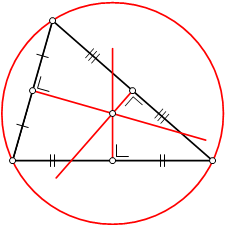
\includegraphics[width=50mm]{./pics/circumcenter.png}
  \end{center}

  \item El baricentro (centro de gravedad) es el punto de intersección de las medianas (recta de un vértice al punto medio del lado opuesto).

  \begin{center}
    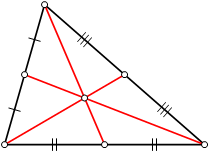
\includegraphics[width=50mm]{./pics/barycenter.png}
  \end{center}

  \item El incentro (centro del círculo inscrito) es el punto de intersección de las bisectrices (recta que divide el ángulo en dos ángulos iguales).

  \begin{center}
    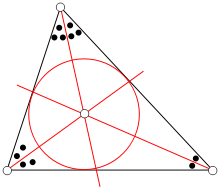
\includegraphics[width=50mm]{./pics/incenter.png}
  \end{center}

  \item El ortocentro es el punto donde se cortan las tres alturas (recta desde un vértice y perpendicular al lado opuesto). El ortocentro se encuentra dentro del triángulo si éste es acutángulo, coincide con el vértice del ángulo recto si es rectángulo, y se halla fuera del triángulo si es obtusángulo.
  
  \begin{center}
    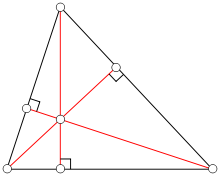
\includegraphics[width=50mm]{./pics/orthocenter.png}
  \end{center}
\end{itemize}

\subsubsection{Centro del círculo que pasa por 3 puntos (circuncentro)}
\small
\textbf{Field-testing:}
\begin{itemize}
\item \emph{Live Archive} - 4807 - Cocircular Points
\end{itemize}
\normalsize

\codigofuente{./src/geometria/circle_through_3_points.cpp}

\subsubsection{Ley del seno y ley del coseno}

\begin{center}
  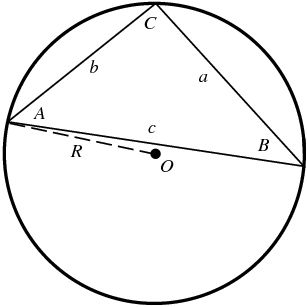
\includegraphics[width=70mm]{./pics/law_of_sines.png}
\end{center}

Sean $a$, $b$ y $c$ las longitudes de los lados de un tríangulo con ángulos opuestos $A$, $B$  y $C$.
La ley del seno dice:

$$
\dfrac{a}{\sin A} = \dfrac{b}{\sin B} = \dfrac{c}{\sin C} = 2R
$$

donde $R$ es el radio del circuncírculo.

Otros resultados son:

$$ a(\sin B - \sin C) + b(\sin C - \sin A) + c(\sin A - \sin B) = 0 $$
$$a = b \cos C + c \cos B$$.

La ley del coseno:

$$ \cos A = \dfrac{c^2 + b^2 - a^2}{2bc} $$

y la ley de tangentes:

$$ \dfrac{a + b}{a - b} = \dfrac{  \tan [\frac{1}{2}(A + B)] }{  \tan [\frac{1}{2}(A - B)]  }. $$

\subsection{Área de un polígono}
Si P es un polígono simple (no se intersecta a sí mismo) su área está dada por:

$$ A(P) = \frac{1}{2} \displaystyle\sum_{i=0}^{n-1} (x_{i} \cdot y_{i+1} - x_{i+1} \cdot y_{i}) $$

\bigskip
\codigofuente{./src/geometria/polygon_area.cpp}

\subsection{Centro de masa de un polígono}
Si P es un polígono simple (no se intersecta a sí mismo) su centro de masa está dado por:


$$ \displaystyle\bar{C}_{x} = \frac{ \displaystyle\iint_{R} x \, dA }{M} = \frac{1}{6M}\sum_{i=1}^{n} (y_{i+1} - y_{i}) (x_{i+1}^2 + x_{i+1} \cdot x_{i} + x_{i}^2) $$

\medskip

$$ \displaystyle\bar{C}_{y} = \frac{ \displaystyle\iint_{R} y \, dA }{M} = \frac{1}{6M} \sum_{i=1}^{n} (x_{i} - x_{i+1}) (y_{i+1}^2 + y_{i+1} \cdot y_{i} + y_{i}^2) $$

\medskip

Donde $ M $ es el área del polígono.

Otra posible fórmula equivalente:

$$ \displaystyle\bar{C}_{x} = \frac{1}{6A} \sum_{i=0}^{n-1} (x_{i} + x_{i+1}) (x_{i} \cdot y_{i+1} - x_{i+1} \cdot y_{i}) $$

\medskip

$$ \displaystyle\bar{C}_{y} = \frac{1}{6A} \sum_{i=0}^{n-1} (y_{i} + y_{i+1}) (x_{i} \cdot y_{i+1} - x_{i+1} \cdot y_{i}) $$


\subsection{Convex hull: Graham Scan}
\emph{Complejidad:} $ O(n \log_{2}{n}) $
\codigofuente{./src/geometria/grahamscan.cpp}

\subsection{Convex hull: Andrew's monotone chain}
\emph{Complejidad:} $ O(n \log_{2}{n}) $
\codigofuente{./src/geometria/monotonechain.cpp}

\subsection{Mínima distancia entre un punto y un segmento}
\codigofuente{./src/geometria/distance_point_to_segment.cpp}

\subsection{Mínima distancia entre un punto y una recta}
\codigofuente{./src/geometria/distance_point_to_line.cpp}

\subsection{Determinar si un polígono es convexo}
\codigofuente{./src/geometria/is_convex_polygon.cpp}

\subsection{Determinar si un punto está dentro de un polígono convexo}
\codigofuente{./src/geometria/is_inside_convex_polygon.cpp}

\subsection{Determinar si un punto está dentro de un polígono cualquiera}
\small
\textbf{Field-testing:}
\begin{itemize}
\item \emph{TopCoder} -  SRM 187 - Division 2 Hard - PointInPolygon
\item \emph{UVa} - 11665 - Chinese Ink
\end{itemize}
\normalsize
\codigofuente{./src/geometria/is_inside_concave_polygon.cpp}

\subsection{Hallar la intersección de dos rectas}
\codigofuente{./src/geometria/line_line_intersection.cpp}

\subsection{Hallar la intersección de dos segmentos de recta}
\label{hallar_interseccion_segmentos}
\small
\textbf{Field-testing:}
\begin{itemize}
\item \emph{UVa} - 11665 - Chinese Ink
\end{itemize}
\normalsize

\codigofuente{./src/geometria/segment_segment_intersection.cpp}

\subsection{Determinar si dos segmentos de recta se intersectan o no}

Si sólo se necesita determinar si dos segmentos se intersectan, pero no hallar
el punto de intersección, se puede usar este código que es más corto que \ref{hallar_interseccion_segmentos}.
La función \verb!point_in_box! es la misma que en \ref{hallar_interseccion_segmentos}.

\codigofuente{./src/geometria/check_segment_intersection.cpp}

\subsection{Cortar un polígono convexo por una recta infinita}

\small
\textbf{Field-testing:}
\begin{itemize}
\item \emph{UVa} - 12514 - Cookie
\end{itemize}
\normalsize

\codigofuente{./src/geometria/split_convex_polygon.cpp}

\subsection{Proyección de un vector en otro}

$$
\vec a \text{ proyectado en } \vec b = \vec c = \dfrac{\vec a \cdot \vec b}{|{\vec b}^2|} \vec b = \dfrac{\vec a \cdot \vec b}{\vec b \cdot \vec b} \vec b. $$

$\vec c$ es un vector nulo ó paralelo a $\vec b$ cuya magnitud es la ``sombra'' (la proyección ortogonal) proyectada por el vector $\vec a$ sobre una recta infinita paralela a $\vec b$. Si $\theta$ es el ángulo entre $\vec a$ y $\vec b$ entonces:

\begin{itemize}
    \item $\vec c = \vec 0$ si $\theta = 90^{\circ}, $
    \item $\vec c$ tiene la misma dirección que $\vec b$ si $0 \leq \theta < 90^{\circ}, $
    \item $\vec c$ tiene dirección contraria a $\vec b$ si $90 < \theta \leq 180^{\circ}. $
\end{itemize}

\subsection{Reflejar un rayo de luz en un espejo}

\textbf{Field-testing:}
\begin{itemize}
\item \emph{Live Archive} - 5929 - Laser Tag
\end{itemize}

Dado un rayo $\vec a$ incidente en una superficie con vector normal unitario $\vec n$ se quiere encontrar el rayo $\vec b$ reflejado en ese punto:


\begin{center}
    \begin{tabular}{ >{\centering\arraybackslash} m{4cm} >{\centering\arraybackslash} m{4cm} }
     \includegraphics{./pics/reflected_ray.1} & $ \vec b = \vec a - 2 (\vec a \cdot \vec n) \vec n $\\
    \end{tabular}
\end{center}

donde $\cdot$ es producto punto. ¡Para que la fórmula funcione $\vec n$ tiene que ser unitario! Notar que no importa cuál de las dos direcciones tiene $\vec n$ porque si lo reemplazamos por $-\vec n$ da el mismo resultado.


\codigofuente{./src/geometria/reflect_ray.cpp}

\subsection{Reflejar un punto al otro lado de una recta}

\textbf{Field-testing:}
\begin{itemize}
\item \emph{Live Archive} - 5929 - Laser Tag
\end{itemize}


\begin{center}
    \includegraphics{./pics/reflected_point.1}
\end{center}

\codigofuente{./src/geometria/reflect_point.cpp}

\subsection{Hallar la intersección de un segmento y una superfice cuádrica (esfera, cono, elipsoide, hiperboloide o paraboloide)}

\textbf{Field-testing:}
\begin{itemize}
\item \emph{UVa} - 11334 - Antenna in the Cinoc Mountains
\end{itemize}

La ecuación genérica para describir una superficie cuádrica es

$$ ax^2 + by^2 + cz^2 + dxy + exz + fyz + gx + hy + iz + j = 0 $$

Se tiene un segmento de $P$ a $Q$ y se quiere hallar la intersección (si existe):

\codigofuente{./src/geometria/segment_quadric_intersection.cpp}

Estas son las ecuaciones de las cónicas más comunes:

% Las ecuaciones están aquí: http://www.professores.uff.br/hjbortol/arquivo/2007.1/qs/quadric-surfaces_br.html

\begin{itemize}
    \item \emph{Elipsoide}: $$ \frac{x^2}{a^2} + \frac{y^2}{b^2} + \frac{z^2}{c^2} = 1.$$
    $a$, $b$ y $c$ son los  ``radios'' en cada dirección (cuando $a = b = c$ se tiene una esfera).
    \item \emph{Paraboloide elíptico}: $$ \frac{x^2}{a^2} + \frac{y^2}{b^2} - z = 0.$$ (Cuando $a = b$ se tiene un paraboloide circular).
    \item \emph{Paraboloide hiperbólico} (\small{silla de montar o papa Pringles}): $$ \frac{x^2}{a^2} - \frac{y^2}{b^2} - z = 0.$$.
    \item \emph{Hiperboloide de una hoja}: $$ \frac{x^2}{a^2} + \frac{y^2}{b^2} - \frac{z^2}{c^2} = 1.$$
    \item \emph{Hiperboloide de dos hojas}: $$ \frac{x^2}{a^2} + \frac{y^2}{b^2} - \frac{z^2}{c^2} = -1.$$
    \item \emph{Cono}: $$ \frac{x^2}{a^2} + \frac{y^2}{b^2} - \frac{z^2}{c^2} = 0.$$ (Cuando $a = b$ se tiene un cono circular).
    
    \begin{tikzpicture}
    \begin{axis}[
        domain=0:5,
        y domain=0:2*pi,
        xmin=-10,
        xmax=10,
        ymin=-10,
        ymax=10,
        samples=20]
    \addplot3 [mesh,draw=black,z buffer=sort,samples=20] 
        ({x*cos(deg(y))},
         {x*sin(deg(y))},
         {x});
    \addplot3 [mesh,draw=black,z buffer=sort] 
        ({x*cos(deg(y))},
         {x*sin(deg(y))},
         {-x});
    \end{axis}
    \end{tikzpicture}.
    
    Para mover el cono se puede usar la ecuación $$ \frac{(x - x_0)^2}{a^2} + \frac{(y - y_0)^2}{b^2} - \frac{(z - z_0)^2}{c^2} = 0$$ aunque generalmente es más fácil trasladar todos los objetos tal que el ápice del cono quede en el origen. Para cambiar el eje en el que se abre el cono, se cambia el signo menos en la ecuación y se pone en frente del eje sobre el que se quiere abrir. Para un cono que se abre en $\mathcal{Z}$ y que tiene radio $r$ a la altura $h$ (como en \emph{Antenna in the Cinoc Mountains}) se usa la ecuación $ \displaystyle x^2 + y^2 = (\frac{r}{h}z)^2.$
    
    \item \emph{Cilindro elíptico}: $$ \frac{x^2}{a^2} + \frac{y^2}{b^2} = 1.$$ (Cuando $a = b$ se tiene un cilindro circular).
    \item \emph{Planos que se intersectan}: $$ \frac{x^2}{a^2} - \frac{y^2}{b^2} = 0. $$
    
\end{itemize}


\subsection{Hallar el área de la unión de varios rectángulos}
\label{area_union_rectangulos}

\textbf{Field-testing:}
\begin{itemize}
\item \emph{TopCoder} - SRM 444 Div 1 Hard - PaperAndPaint
\end{itemize}

\codigofuente{./src/geometria/rectangles_union_area.cpp}

\subsection{Hallar el volumen de la unión de varios parelelepípedos}

\textbf{Field-testing:}
\begin{itemize}
\item \emph{Live Archive} - 4969 - World of cubes
\end{itemize}

Necesita también el código de la unión de rectángulos (sección \ref{area_union_rectangulos}).

\codigofuente{./src/geometria/parallelepiped_union_volume.cpp}

\subsection{Mínima distancia entre dos puntos en la superficie de la Tierra}
\small
\textbf{Field-testing:}
\begin{itemize}
\item \emph{UVa} - 535 - Globetrotter
\end{itemize}
\normalsize

\codigofuente{./src/geometria/great_circle_distance.cpp}

\subsection{Distancias más cortas en 3D (punto a segmento, segmento a segmento y punto a triángulo)}
\small
\textbf{Field-testing:}
\begin{itemize}
\item \emph{UVa} - 11836 - Star War
\end{itemize}
\normalsize

\codigofuente{./src/geometria/shortest_distances_in_3d.cpp}

\subsection{Punto más cercano de aproximación}

Supongamos que en el tiempo $t = 0$ el avión 1 está en $P_0$ y el avión 2 está en $Q_0$ 
y sus vectores de velocidad por unidad de tiempo son $\vec{u}$ y $\vec{v}$ respectivamente.

Las posiciones de cada avión en el tiempo $t$ están dadas por $P(t) = P_0 + t \vec{u}$ y
$Q(t) = Q_0 + t \vec{v}$.

Llamemos $\vec{w_0} = P_0 - Q_0$. Entonces el instante de tiempo en que los dos aviones están lo más cerca posible está
dado por:

$$
t_c = \dfrac{-\vec{w_0} \cdot (\vec{u} - \vec{v}) }{ |\vec{u} - \vec{v}|^2 }
$$

siempre y cuando $|\vec{u} - \vec{v}|$ no sea 0. Si $|\vec{u} - \vec{v}| = 0$, los
dos aviones viajan en la misma dirección a la misma velocidad y siempre van a estar
a la misma distancia, entonces se puede simplemente usar $t_c = 0$.

Cuando $t_c < 0$, los aviones ya estuvieron lo más cerca posible en el pasado y 
se están alejando cada vez más a medida que avanzan.

\subsection{Círculo más pequeño que envuelve una lista de puntos}
\small
\textbf{Field-testing:}
\begin{itemize}
\item \emph{SPOJ} - ALIENS - Aliens
\end{itemize}
\normalsize

\codigofuente{./src/geometria/minimum_enclosing_circle.cpp}


% ---------------------------------------------------------------
\section{Estructuras de datos}
\subsection{Árboles de Fenwick ó Binary indexed trees}

Se tiene un arreglo $\{a_0, a_1, \cdots, a_{n-1}\}$. Los árboles
de Fenwick permiten encontrar $ \displaystyle \sum_{k=i}^{j} a_k $ en orden $O(\log_{2}{n})$ para parejas de $(i, j)$ con $i \leq j$. De la misma manera, permiten sumarle una cantidad a un $a_i$ también en tiempo $O(log_{2}{n})$.
\medskip
\codigofuente{./src/estructuras/fenwick.cpp}

\subsection{Segment tree}
\codigofuente{./src/estructuras/segment_tree.cpp}

\subsection{Treap}
\codigofuente{./src/estructuras/treap.cpp}

\subsection{Rope}
\codigofuente{./src/estructuras/rope.cpp}

\subsection{Range Minimum Query}
\subsubsection{Con tabla}
\codigofuente{./src/estructuras/rmq/rmq_with_table.cpp}
\subsubsection{Con segment tree}
\codigofuente{./src/estructuras/rmq/rmq_with_segment_tree.cpp}


% ---------------------------------------------------------------
\section{Misceláneo}

\subsection{Problema de Josephus}

Hay $n$ personas enumeradas de $0$ a $n - 1$ paradas en un círculo. Un verdugo empieza a contar personas en sentido horario, empezando en la persona $0$. Cuando la cuenta llega a $k$, el verdugo mata a la última persona contada y vuelve a empezar a contar a partir siguiente persona. ¿Quién es el sobreviviente?

Por ejemplo, si $n = 7$ y $k = 3$, el orden en que se eliminan las personas es 2, 5, 1, 6, 4, 0 y 3. El sobreviviente es 3.

\codigofuente{./src/misc/josephus.cpp}

\subsection{Distancia más corta para un caballo en un tablero de ajedrez infinito}

\codigofuente{./src/misc/knight_distance.cpp}

\subsection{Trucos con bits}
\subsubsection{Iterar sobre los subconjuntos de una máscara}

\codigofuente{./src/misc/subsets_of_mask.cpp}

\subsection{El \textit{parser} más rápido del mundo}
\begin{itemize}
\item Cada no-terminal: un método
\item Cada lado derecho:
  \begin{itemize}
  \item invocar los métodos de los no-terminales o
  \item Cada terminal: invocar proceso \textit{match}
  \end{itemize}
\item Alternativas en una producción: se hace un \textit{if}
\end{itemize}
\medskip
No funciona con gramáticas recursivas por izquierda ó en las que en algún momento haya
varias posibles escogencias que empiezan por el mismo caracter (En ambos casos la gramática se puede factorizar).

\medskip
\textbf{Ejemplo:} Para la gramática:
$$
A \longrightarrow (A)A
$$ $$
A \longrightarrow \epsilon
$$

\codigofuente{./src/misc/parser_recursivo_desc.cpp}

\subsection{Checklist para corregir un Wrong Answer}
Consideraciones que podrían ser causa de un Wrong Answer:
\begin{itemize}
  \begin{item}
    Overflow.
  \end{item}

  \begin{item}
    El programa termina anticipadamente por la condición en el ciclo de lectura.
    Por ejemplo, se tiene \verb_while (cin >> n >> k && n && k)_ y un caso válido de entrada
    es n = 1 y k = 0.
  \end{item}

  \begin{item}
    El grafo no es conexo.
  \end{item}

  \begin{item}
    Puede haber varias aristas entre el mismo par de nodos.
  \end{item}

  \begin{item}
    Las aristas pueden tener costos negativos.
  \end{item}

  \begin{item}
    El grafo tiene un sólo nodo.
  \end{item}

  \begin{item}
    La cadena puede ser vacía.
  \end{item}

  \begin{item}
    Las líneas pueden tener espacios en blanco al principio o al final (Cuidado al usar \texttt{getline} o \texttt{fgets}).
  \end{item}

  \begin{item}
    El arreglo no se limpia entre caso y caso.
  \end{item}

  \begin{item}
    Estás imprimiendo una línea en blanco con un espacio (\verb_printf(" \n")_ en vez de \verb_printf("\n")_  ó \verb_puts(" ")_  en vez de \verb_puts("")_).
  \end{item}

  \begin{item}
    Hay pérdida de precisión al leer variables como \verb_double_ y convertirlas a enteros. Por ejemplo, en C++, \verb_floor(0.29 * 100) == 28_.
  \end{item}

  \begin{item}
    La rana se puede quedar quieta.
  \end{item}
  
  \begin{item}
    El producto cruz está invertido. Realmente es $$|\langle a_x, a_y \rangle \times \langle b_x, b_y\rangle| = a_x \mathbf{b_y} - a_y \mathbf{b_x} \neq a_x \mathbf{b_x} - a_y \mathbf{b_y}. $$
  \end{item}
  
  \begin{item}
      Hay una resta módulo $m$ pero no se revisa si el resultado es negativo. Se corrige haciendo \begin{verbatim}
      ans = (ans - b) % mod;
      if (ans < 0) ans += mod;   // !
\end{verbatim}.
  \end{item}
\end{itemize}

\subsection{Redondeo de dobles}

Para redondear un doble a $k$ cifras, usar:

$$ \dfrac{\lfloor 10^{k} \cdot x + 0.5 \rfloor }{10^k} $$

Ejemplo:
\begin{verbatim}
  double d = 1.2345;
  d = floor(1000 * d + 0.5) / 1000;
\end{verbatim}

Al final, \verb_d_ es 1.235.

\subsubsection{Convertir un doble al entero más cercano}

\begin{center}
  \renewcommand{\arraystretch}{1.3} %Multiplica la altura de cada fila de la tabla por 2
  % Si quiero aumentar el tamaño de una fila en particular insertar \rule{0cm}{1cm} en esa fila.
  \begin{tabular}{| c | c | c | }
    \hline
    \textit{Código} & \textit{Valores originales ($d$)} & \textit{Nuevos valores ($k$)} \\
    \hline\hline

    \verb_int k = floor(d + 0.5 + EPS);_ & 0.0  & 0 \\ \cline{2-3}
    (con \verb_EPS = 1e-9_)              & 0.1  & 0 \\ \cline{2-3}
                                         & 0.5  & 1 \\ \cline{2-3}
                                         & 0.4999999999999999 & 1 \\ \cline{2-3}
                                         & \verb_cos(1e-7) * 0.5_ =  & \\ & 0.4999999999999975 & 1 \\ \cline{2-3}
                                         & 0.9  & 1 \\ \cline{2-3}
                                         & 1.0 & 1 \\ \cline{2-3}
                                         & 1.4 & 1 \\ \cline{2-3}
                                         & 1.5 & 2 \\ \cline{2-3}
                                         & 1.6 & 2 \\ \cline{2-3}
                                         & 1.9 & 2 \\ \cline{2-3}
                                         & 2.0 & 2 \\ \cline{2-3}
                                         & 2.1 & 2 \\ \cline{2-3}
                                         & -0.0  & 0 \\ \cline{2-3}
                                         & -0.1  & 0 \\ \cline{2-3}
                                         & -0.5  & 0 \\ \cline{2-3}
                                         & -0.4999999999999999 & 0 \\ \cline{2-3}
                                         & \verb_-cos(1e-7) * 0.5_ =  & \\ & -0.4999999999999975 & 0 \\ \cline{2-3}
                                         & -0.9  & -1 \\ \cline{2-3}
                                         & -1.0 & -1 \\ \cline{2-3}
                                         & -1.4 & -1 \\ \cline{2-3}
                                         & -1.5 & -1 \\ \cline{2-3}
                                         & -1.6 & -2 \\ \cline{2-3}
                                         & -1.9 & -2 \\ \cline{2-3}
                                         & -2.0 & -2 \\ \cline{2-3}
                                         & -2.1 & -2 \\ \cline{2-3}
    \hline
  \end{tabular}
  \renewcommand{\arraystretch}{1}
\end{center}

\begin{center}
  \renewcommand{\arraystretch}{1.3} %Multiplica la altura de cada fila de la tabla por 2
  % Si quiero aumentar el tamaño de una fila en particular insertar \rule{0cm}{1cm} en esa fila.
  \begin{tabular}{| c | c | c | }
    \hline
    \textit{Código} & \textit{Valores originales ($d$)} & \textit{Nuevos valores ($k$)} \\
    \hline\hline

    \verb_int k = floor(d + 0.5);_       & 0.0  & 0 \\ \cline{2-3}
                                         & 0.1  & 0 \\ \cline{2-3}
                                         & 0.5  & 1 \\ \cline{2-3}
                                         & 0.4999999999999999 & 0 \\ \cline{2-3}
                                         & \verb_cos(1e-7) * 0.5_ =  & \\ & 0.4999999999999975 & 0 \\ \cline{2-3}
                                         & 0.9  & 1 \\ \cline{2-3}
                                         & 1.0 & 1 \\ \cline{2-3}
                                         & 1.4 & 1 \\ \cline{2-3}
                                         & 1.5 & 2 \\ \cline{2-3}
                                         & 1.6 & 2 \\ \cline{2-3}
                                         & 1.9 & 2 \\ \cline{2-3}
                                         & 2.0 & 2 \\ \cline{2-3}
                                         & 2.1 & 2 \\ \cline{2-3}
                                         & -0.0  & 0 \\ \cline{2-3}
                                         & -0.1  & 0 \\ \cline{2-3}
                                         & -0.5  & 0 \\ \cline{2-3}
                                         & -0.4999999999999999 & 0 \\ \cline{2-3}
                                         & \verb_-cos(1e-7) * 0.5_ =  & \\ & -0.4999999999999975 & 0 \\ \cline{2-3}
                                         & -0.9  & -1 \\ \cline{2-3}
                                         & -1.0 & -1 \\ \cline{2-3}
                                         & -1.4 & -1 \\ \cline{2-3}
                                         & -1.5 & -1 \\ \cline{2-3}
                                         & -1.6 & -2 \\ \cline{2-3}
                                         & -1.9 & -2 \\ \cline{2-3}
                                         & -2.0 & -2 \\ \cline{2-3}
                                         & -2.1 & -2 \\ \cline{2-3}
    \hline
  \end{tabular}
  \renewcommand{\arraystretch}{1}
\end{center}

\subsubsection{Redondear un doble a cierto número de cifras de precisión}


\section{Java}
\subsection{Entrada desde entrada estándar}
Este primer método es muy fácil pero es mucho más ineficiente porque utiliza Scanner en vez de BufferedReader:
\codigofuente{./src/java/io_estandar_easy.java}

\bigskip

Este segundo es más rápido:
\codigofuente{./src/java/io_estandar.java}
\subsection{Entrada desde archivo}
\codigofuente{./src/java/io_file.java}

\subsection{Mapas y sets}
Programa de ejemplo:
\codigofuente{./src/java/maps_sets.java} \\
La salida de este programa es: \\
\bigskip
\ttfamily
\fbox{\parbox{5.0cm}{
    Maps\\
    m.size() = 1\\
    465\\
    null\\
    \\
    Sets\\
    54 presente.\\
    s.size() = 3\\
    54\\
    3576\\
    1000000007\\
    s.size() = 0
  }
}
\normalfont\normalsize
\bigskip

Si quiere usarse una clase propia como llave del mapa o como elemento del set, la clase debe implementar
algunos métodos especiales: Si va a usarse un TreeMap ó TreeSet hay que implementar los métodos \texttt{compareTo} y
\texttt{equals} de la interfaz \texttt{Comparable} como en la sección \ref{colas_de_prioridad_java}. Si va a usarse
un HashMap ó HashSet hay más complicaciones.\\
\smallskip
\textbf{Sugerencia:} Inventar una manera de codificar y decodificar la clase en una String o un Integer y meter esa representación en el mapa o set: esas clases ya tienen los métodos implementados.

\subsection{Colas de prioridad}
\label{colas_de_prioridad_java}
Hay que implementar unos métodos. Veamos un ejemplo:

\smallskip

\codigofuente{./src/java/priority_queue.java}

\smallskip

La salida de este programa es:

\smallskip

\ttfamily
\fbox{\parbox{5.0cm}{
    peso = 0, destino = 12\\
    peso = 0, destino = 8\\
    peso = 0, destino = 13\\
    peso = 3, destino = 7\\
    peso = 1876, destino = 4
  }
}
\normalfont\normalsize

\medskip

Vemos que la función de comparación que definimos no tiene en cuenta \texttt{destino},
por eso no desempata cuando dos \texttt{Items} tienen el mismo \texttt{peso} si no que escoge
cualquiera de manera arbitraria.

\section{C++}
\subsection{Entrada desde archivo}
\codigofuente{./src/c++/io_file.cpp}

\subsection{Strings con caractéres especiales}
\codigofuente{./src/c++/unicode.cpp}

\emph{Nota}: Como alternativa a la función getline, se pueden utilizar las funciones fgetws y fputws, y más adelante swscanf y wprintf:
\codigofuente{./src/c++/fgetws.cpp}

\subsection{Imprimir un doble con \texttt{cout} con cierto número de cifras de precisión}
Tener cuidado con números negativos, porque el comportamiento es diferente.

\codigofuente{./src/c++/cout_con_precision.cpp}

\end{document}